% LaTeX source for interim report
\documentclass[a4paper,11pt]{article}
\usepackage[margin=1in]{geometry}
\usepackage{hyperref}
\usepackage{parskip}  % add space between paragraphs
\usepackage{graphicx}
\usepackage{float}

% Title and Author
\title{Asymmetric Communication Policies in\\Multi-Agent Reinforcement Learning for Tethered Robots}
\author{Chintan Shah}
\date{\08 April, 2025}

\begin{document}

\maketitle
\clearpage

\begin{abstract}
This report describes the progress made in implementing asymmetric communication policies using the enhanced encoder-decoder architecture and tether violation handling. Supported by several performance plots, it reflects on the design evolution since the proposal stage and covers the gaps in our presentation from the architectural, experimental, and training modifications aspects. Given our intention to achieve publishable results, it serves as an interim documentation.
\end{abstract}

\section{Project Background}
Setting in a grid where agents with different roles must reach the target within the least possible steps, our project aims to research and develop effective communication strategies given partial observability. With the difficulty of learning an effective protocol in one-way transmissions, our solutions are based on decentralized execution while taking the benefit from a shared critic network.

\section{Environment Resetting}
In our design, the environment is reset if an agent attempts to go out of its predefined tether limit. The problem happens during training processes, where we noticed many episodes being reset, partly because of out-of-tether situations, out-of-bound situations, colliding with another agent, or bumping into a hard obstacle. As a result, we proposed a solution. In such situations, if it is in a “training mode”, we simply penalize the agent and reverse its move.

This change also incurs a challenge. We penalize agents for staying in the same position, which helps agents minimize movements while reaching the target. We noticed reversing moves counting the penalty as well for staying in the same position, because agents in fact do not move to a new valid position (after their positions being reversed). For example, if an agent tries to go outside the grid, we penalize it with –50 reward, but reversing their positions in “training mode” yields another –3 penalty, which is the one for staying in the same position. Our enhanced solution to that is to reduce the out-of-bound penalty by 3. In this way, it avoids double counting the penalties.

% ——— Specific Scenario: Tether Management ———
\section{Specific Scenario – Tether Management}

Robots maintaining within the tether, a predefined fixed distance throughout their entire trajectories, is the focus of our project. This is also an extension to the idea of relaxing constraints of environment resetting, but particularly on out‑of‑tether scenarios. The goal here is to help agents learn to minimize tether violations by introducing severe penalties in such a type of scenario.

Initially, we only penalized agents in such a scenario with a –50 reward. However, this is the same magnitude as the penalty for other undesirable events, which proved insufficient given our intention to train agents to incur the fewest tether violations. Hence, we developed the following enhanced scheme:

\begin{enumerate}
  \item Obtain the tether limit \(d_{\max}\) (a configurable environment parameter).
  \item During each episode, count the number of tether violations \(v_t\) up to time \(t\).
  \item In \emph{training mode} (where the environment does not reset immediately), apply a scaled penalty each time a violation occurs:
  \[
    r_t^{\rm tether} \;=\; -50 \;-\; \beta \, v_t
  \]
  Here \(\beta\) is a tunable severity factor (e.g.\ \(\beta=10\)) and \(v_t\) is the cumulative violation count so far.
  \item Continue the episode (do not reset) until a \emph{tether toleration count} \(V_{\rm tol}\) is exceeded.  We currently hard‑code \(V_{\rm tol}=5\); after \(v_t>V_{\rm tol}\), the episode is finally reset even in training mode.
\end{enumerate}

For deployment (execution) mode, any tether violation still triggers an immediate environment reset—so this penalty scheme affects only the learning dynamics, encouraging agents to avoid repeated violations rather than merely reset and try again.

\bigskip
\noindent\textbf{Hyperparameters to tune:}
\begin{itemize}
  \item \(\beta\) (penalty scaling per violation)
  \item \(V_{\rm tol}\) (maximum tolerated violations per episode)
\end{itemize}

\section{Experimental Analysis}

We prepared a systematic pipeline for efficient training and debugging, involving an initialization of the SimpleGrid-based environment, the creation of a grid search, the backpropagation of weights and gradients, an evaluation and logging, which is shown in the appendix section. 

Figure 1 shows the Gradient change over the episodes. Before episode 15, the gradient fluctuates, indicating that the model is still exploring different strategies and adjusting its parameters. During this phase, the model likely experiences exploration-heavy behavior and might not have settled on the most efficient policy yet. After episode 15, the gradient appears to stabilize. This could indicate that the model is starting to converge, reducing fluctuations in its learning. The agent may have learned more consistent strategies by this point, which results in lower and less variable gradient changes. There is a significant spike in the gradient change around episode 30 which suggests a sudden change in the model’s learning behavior at this point. It shows instability during training. Ignoring this spike, the gradient changes after episode 30 seem relatively steady. This suggests that despite the anomaly at episode 30, the model’s learning has largely stabilized, and it has reached a state where it is no longer drastically adjusting its weights with each new episode. 

\begin{figure}[H]
    \centering
    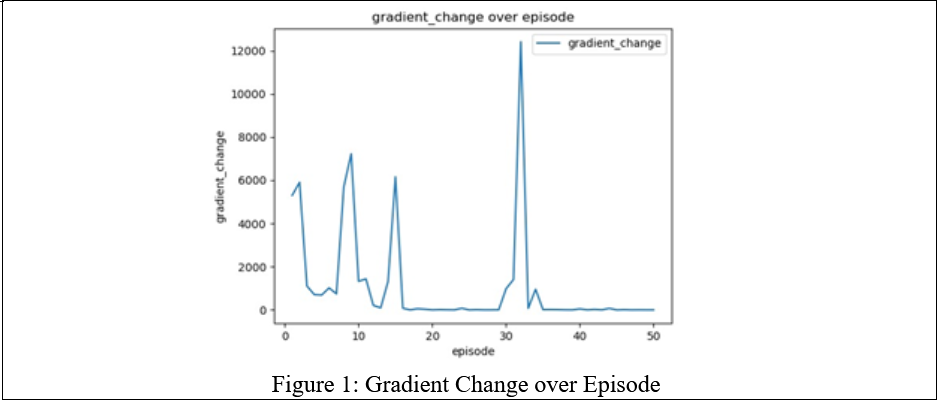
\includegraphics[width=0.75\linewidth]{fig1.png}
    \caption{Gradient Change over Episode}
    \label{fig:enter-label}
\end{figure}


Figure 2 shows the total loss over episodes. The graph shows a drastic dip in the loss around episode 15, followed by some fluctuation. The significant drop could be linked to a sudden improvement in the model’s ability to make decisions, possibly due to better learning of the environment's dynamics or the correct actions. The total loss oscillates after episode 15, suggesting that the model is in the process of stabilizing but still adjusting its parameters. The sharp drop at episode 15 might correspond to a critical moment when the agent learned a key strategy or improved its exploration-exploitation balance. 

\begin{figure}[H]
    \centering
    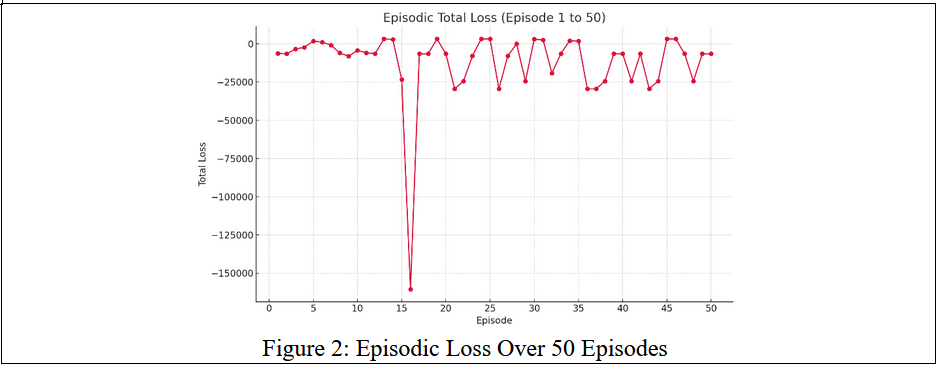
\includegraphics[width=0.75\linewidth]{fig2.png}
    \caption{Episodic Loss Over 50 Episodes}
    \label{fig:enter-label}
\end{figure}

Figure 3 Shows the reward over episode. There is a sudden, dramatic drop in reward around episode 15. This suggests that the agents may have faced a significant penalty or failure at this point. This drop aligns with the previous loss graph's sharp changes which suggests a strong negative outcome in the training process during this episode. Prior to episode 15, rewards seem relatively stable, with small fluctuations. This could indicate that the agents are not performing consistently at this stage, possibly still learning and exploring. After the sharp drop in episode 15, the rewards stabilize that shows smaller and less dramatic changes. This could be a sign that the agents are starting to perform more consistently and are refining their strategies. 

\begin{figure}
    \centering
    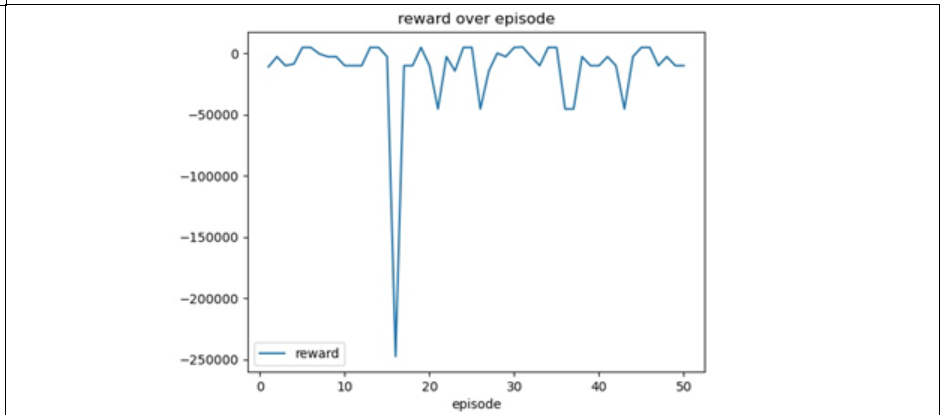
\includegraphics[width=0.75\linewidth]{fig3.png}
    \caption{Cumulative Reward over Episodes}
    \label{fig:enter-label}
\end{figure}

Early on, the agent is exploring the environment, which causes higher gradient fluctuations (seen in the gradient graph). At the same time, the reward graph shows some fluctuations and instability, possibly due to the agent trying out different actions and facing challenges (getting low rewards or penalties). Moreover, the sharp drop in both reward (in episode 15) and gradient change (episode 15-30) suggests that the agent faced a significant challenge, possibly from a failed strategy or an environment state that led to poor performance (with a low reward) and large gradient updates as the model tried to adjust. After episode 15, the gradient stabilizes, and the reward becomes more consistent. This could indicate that the model has learned to optimize its strategy, and as a result, the gradients become smaller (indicating less adjustment needed) and rewards become more stable, reflecting better performance.  

As the model learns, it adjusts its weights based on gradients. The gradient change graph shows how much the model is modifying its weights, which should correspond to the total loss changes. High gradients often happen when the model is far from optimal, and large weight updates are needed, which corresponds to higher total loss values in earlier episodes (around episode 15, where the loss graph shows a big dip). After episode 15, both the gradient and total loss seem to stabilize, suggesting that the model has started learning and reducing its errors, as seen by the decreasing total loss and the steadier gradient. 

Generally, as the reward increases (when the agent performs better), the total loss should decrease because the agent's actions are becoming more optimal. Early in training, the agent is likely to receive lower rewards (shown in the reward graph), which results in higher total loss (with poor performance). As the agent improves and the rewards increase, the total loss decreases, as seen in the smoother, more negative total loss after episode 15. When the reward drops sharply at episode 15, we also see a significant drop in loss. This might suggest that the agent made a significant improvement or adjustment, leading to a better balance between exploration and exploitation, resulting in improved reward and lower loss afterward. 

\section{Enhancing our Encoder-Decoder Architecture }
\subsection{Use of GRU Layer}
Encoding a message is an essential process during communication because this process is supposed to make sure the intended recipient understands what another agent (i.e., the leader) knows within its partial observability. By using LSTM (Long-Short Term Memory) layers, the training time was very long. It took 23 hours to complete the entire training pipeline. As a performance booster, our encoder-decoder architecture With GRU (Gated Recurrent Unit) layers, it took 1 less hour to train (i.e., 22 hours), although the time was still quite long. In our experiment, we proved that using GRU (Gated Recurrent Unit) layers consumes far less training parameters than using LSTM (Long Short-Term Memory) layers. For example, from a layer with a shape of (None, 1, 64), LSTM requires 18,888 parameters in training, whereas GRU requires only 14,208 parameters in training. From another layer with a shape of (None, 32), LSTM requires 12,416 parameters in training, whereas GRU requires only 9408 parameters in training. Using 2 LSTM layers in our encoder model takes in total 31,104 parameters in training with 121.50 KB, while using 2 GRU layers requires only in total 23,616 trainable parameters with 92.25 KB. In those examples, using GRU layers are proven to have faster training time given its advantage of the reduced use of computational resources like memory consumption. By enhancing the performance, we also ensured GRU layers work as intended. With LSTM layers, since they are bi-directional, we could decode the message using the exact same type of layer. With GRU, we applied a RepeatVector layer prior to GRU layers in the decoder model, which ensures that encoded messages could be properly transformed back to the interpretation of a valid leader’s message with the exact same type of GRU layers. Therefore, with GRU layers, we not only guarantee a performance boost, but also guarantee the intended use of layers in the encoder-decoder architecture. 

\section{Maintaining Constant Sizes of Message}
Communication is the crux of the problem. As stated above, we will have to maintain understandability of each transmitted message. We defined the leader’s message size is defined to be an array of 8 numbers, which refers to the following items (in sequence): distance to the nearest obstacle, whether the path is clear or blocked, whether the leader can observe the follower, leader's distance to follower, leader's suggested action in x coordinates, leader's suggested action in y coordinates, leader's current move in x coordinates, and leader's current move in y coordinates. The problem happened to be that our encoder model was enlarging the message’s size from 8 to 32 for no reason. Therefore, we must maintain constant sizes of messages during encoding or decoding processes. The purpose is to guarantee the message’s integrity – a higher chance where the receiver (i.e., the follower agent) could understand correctly and act as expected by the sender (i.e., the leader). Its advantages are proven in our experiment. The following graphs show the reconstruction losses over episodes during training. The “reconstruction loss” refers to how much information is lost during the message transfer. Figure 4 shows that, enlarging the message’s size during encoding yielded a maximum loss of 17.5; while figure 5 shows that, keeping the encoded message’s size = the original leader’s message size only yielded a maximum loss of 2.2. From this comparison, we understand that maintaining constant sizes of messages throughout communication significantly reduces the message’s reconstruction loss effectively.

\begin{figure}
    \centering
    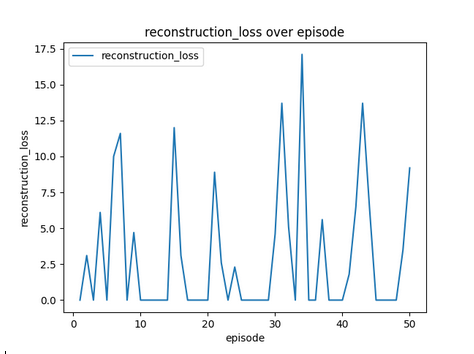
\includegraphics[width=0.5\linewidth]{fig4.png}
    \caption{Episodic Reconstruction Loss when Encoded Message Size = 32 numbers}
    \label{fig:enter-label}
\end{figure}

\begin{figure}
    \centering
    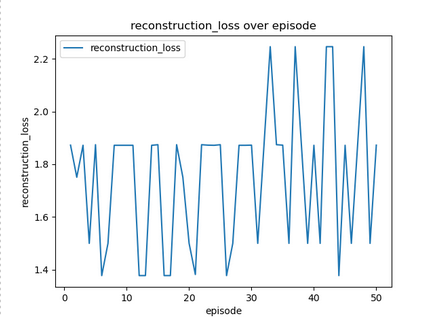
\includegraphics[width=0.5\linewidth]{fig5.png}
    \caption{Episodic Reconstruction Loss when Encoded Message Size = 8 numbers  = Leader’s Original Message Size }
    \label{fig:enter-label}
\end{figure}

\section{Future Work}
\subsection{Model Adjustment}
In the subsequent phase of the project, we are going to adjust the model, in the following aspects: 

    Adjusting hyper-parameters such as learning rate for gradual stabilization in Gradients, 

    Implementing reward shaping to handle the sharp drop in reward function, 

    Fine-tuning the loss components to handle the total loss oscillation. 

\subsection{The DIAL Method}
As mentioned in the presentation, we intend to implement further communication protocols like the DIAL (Differentiable Inter-Agent Learning) method. With a decentralized design and the parameter-sharing scheme, we identified 2 technical improvements in the performance in our presentation, namely the use of GRU layers and a Gumbel Softmax (activation) Layer. As a result, we presented some proof-of-concept codes on our code repository.

\subsection{Bayesian Probabilities}
Chalkiadakis and Boutilier ​(Georgios Chalkiadakis, Craig Boutilier, 2003)​ proposes a Bayesian model-based MARL framework that helps agents achieve the following goals: 

    Balance exploration and exploitation, 

    Learn not only environment dynamics but also other agents’ strategy models, and 

    Use value of information (VOI) to select actions that maximize expected long-term payoff, considering how their actions affect others. 

It is powerful in identical interest games, which align with our asymmetric settings, where both the leader and follower agents share a common goal – reaching the target within minimal steps.  

The theory behind in short mainly involves transitions between Markov Decision Processes (MDP). As a result, agents will take history movements into their memories while making a decision on the current state. It is believed to boost performance compared to existing models which heavily relies on computations solely on the current state.

\section{Conclusion}
Within the timeline of the course, we successfully implemented a baseline model based on MAPPO (Multi-Agent Proximal Policy Optimization). We also successfully integrated it with agents and the environment. To achieve publishable results, however, there is still much work to be done to research, experiment and implement a wider variety of algorithms and models, as well as to integrate a fully functional (and trained) model into agents and the environment. 

\end{document}
